\documentclass[11pt,letterpaper]{article}
\usepackage[margin=.68in,headheight=14pt]{geometry}
\usepackage[T1]{fontenc}\usepackage{lmodern,microtype,amsmath,amssymb,enumitem,xcolor,fancyhdr,tabularx,booktabs,tikz,tcolorbox}
\usetikzlibrary{arrows.meta}
\definecolor{olive}{HTML}{4D5430}\definecolor{gold}{HTML}{9A7B22}\definecolor{pale}{HTML}{F5F1DC}\definecolor{softgreen}{HTML}{EDF0E2}\definecolor{softgray}{HTML}{F5F5F2}\definecolor{ink}{HTML}{292D20}
\color{ink}\pagestyle{fancy}\fancyhf{}\lhead{\textcolor{olive}{MATH\& 107: Math in Society}}\rhead{\textcolor{gold}{Module 8 / Fall 2026}}\cfoot{\thepage}\setlength{\parindent}{0pt}\setlength{\parskip}{5pt}
\setlist[enumerate]{leftmargin=*,itemsep=7pt,topsep=5pt}
\newtcolorbox{keybox}[1]{colback=pale,colframe=olive,boxrule=.7pt,arc=1.5mm,title=\textbf{#1},fonttitle=\color{olive},left=2mm,right=2mm,top=1.5mm,bottom=1.5mm}
\newtcolorbox{examplebox}[1]{colback=softgreen,colframe=gold,boxrule=.7pt,arc=1.5mm,title=\textbf{#1},fonttitle=\color{ink},left=2mm,right=2mm,top=1.5mm,bottom=1.5mm}
\newcommand{\phead}[2]{\clearpage{\Large\bfseries\textcolor{olive}{Module 8: Graph Theory and Networks — #1}}\par\vspace{2pt}\textcolor{gold}{\rule{\linewidth}{1.2pt}}\par\smallskip #2\par}
\newcommand{\name}{Name: \rule{2.6in}{.35pt}\hfill Date: \rule{1.2in}{.35pt}\par}
\newcommand{\work}[1]{\par\vspace{#1}}
\tikzset{n/.style={circle,draw=olive,fill=olive!13,thick,minimum size=8mm,inner sep=0pt,font=\bfseries},e/.style={draw=olive,thick},broken/.style={draw=red!60,very thick,dashed}}
\newcommand{\smallnet}{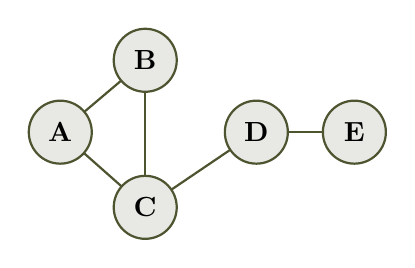
\begin{tikzpicture}[scale=.83,baseline=(current bounding box.center)]
\coordinate(A)at(0,1.15);\coordinate(B)at(1.3,2.25);\coordinate(C)at(1.3,0);\coordinate(D)at(3,1.15);\coordinate(E)at(4.5,1.15);
\foreach\a/\b in {A/B,A/C,B/C,C/D,D/E}{\draw[e](\a)--(\b);}\foreach\v in{A,B,C,D,E}{\node[n] at(\v){\v};}\end{tikzpicture}}
\newcommand{\checknet}{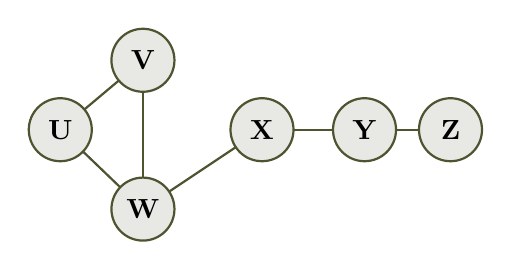
\begin{tikzpicture}[scale=.84,baseline=(current bounding box.center)]
\coordinate(U)at(0,1.2);\coordinate(V)at(1.25,2.25);\coordinate(W)at(1.25,0);\coordinate(X)at(3.05,1.2);\coordinate(Y)at(4.6,1.2);\coordinate(Z)at(5.9,1.2);
\foreach\a/\b in {U/V,U/W,V/W,W/X,X/Y,Y/Z}{\draw[e](\a)--(\b);}\foreach\v in{U,V,W,X,Y,Z}{\node[n] at(\v){\v};}\end{tikzpicture}}
\begin{document}
\phead{Summary}{\textbf{Central idea:} The arrangement of connections determines who can reach whom and whether a system can continue working after a failure.}
\begin{center}\smallnet\end{center}
\begin{keybox}{Represent a network}
A \textbf{node} (vertex) is a place or person. An \textbf{edge} is a direct connection. The graph above has nodes A--E and edges AB, AC, BC, CD, DE. A line that passes near a node without meeting it does not create a connection. The drawing is not a map to scale.
\end{keybox}
\begin{examplebox}{Count direct neighbors}
The \textbf{degree} of C is 3, because it touches A, B, and D. Degrees A--E are 2, 2, 3, 2, 1; their sum is 10. Each of the five edges gets counted at two ends: \(\text{sum of degrees}=2\times\text{number of edges}\).
\end{examplebox}
\begin{keybox}{Paths and distance}
A \textbf{path} travels along existing edges. A--C--D--E uses \textbf{three edges}, so its length is 3. A \textbf{shortest path} uses the fewest edges when links are unweighted. A and E are connected through this path even though they are not direct neighbors. If edges have travel times, add those times instead of counting links.
\end{keybox}
\begin{keybox}{Connected components and bridges}
A \textbf{connected component} is a group in which any node can reach any other. The original graph has one component. If C--D fails, the components are \(\{A,B,C\}\) and \(\{D,E\}\). The edge C--D is a \textbf{bridge}, because removing it separates the graph. By contrast A--B is not a bridge: A and B can still reach each other through C.
\end{keybox}
\phead{Summary (continued)}{\textbf{Use the mathematics to compare choices.}}
\begin{examplebox}{One new link, different outcomes}
Suppose C--D might fail. Adding A--C would not help: that link already exists. Adding B--E creates a new route B--E between the two sides. After C--D fails, A--B--E--D still works. The \textbf{location} of the new edge matters more than the count alone.
\end{examplebox}
\begin{keybox}{An alert moves one link per round}
Begin with A informed in round 0. In each round, informed nodes send to their direct neighbors. Recipients can relay in the \emph{next} round; all direct links work.
\begin{center}\begin{tabular}{@{}cll@{}}\toprule Round & Newly informed & Total informed\\\midrule0&A&A\\1&B, C&A, B, C\\2&D&A, B, C, D\\3&E&A, B, C, D, E\\\bottomrule\end{tabular}\end{center}
With this rule, the first round a node receives an alert equals the shortest-path distance from A. A failed bridge can prevent delivery entirely.
\end{keybox}
\begin{keybox}{A five-step method}
\begin{enumerate}[leftmargin=1.25em,itemsep=2pt]
\item Say what nodes and edges mean in the situation.
\item Decide whether the question concerns direct contacts, routes, failure, or spreading.
\item Count neighbors or trace paths; verify every link exists.
\item Compare the original network with one specific change.
\item Explain a limitation (such as travel time, unreliable contacts, or accessibility).
\end{enumerate}
\end{keybox}
\textbf{Remember:} Two networks can have the same number of edges and very different routes and vulnerabilities. The arrangement matters.
\phead{Prequiz}{\textit{Open-note practice. Show your counts and routes. Brief explanations are enough.}\par\name}
\begin{center}\smallnet\end{center}
Use the graph above for all five questions. Edges: AB, AC, BC, CD, DE.
\begin{enumerate}
\item What are C's direct neighbors? Find the degree of C. Check the handshake rule by adding all five degrees.\work{.58in}
\item Find one shortest path from A to E. Write its nodes in order and give its length in edges. Explain why A and E are connected even though no direct edge joins them.\work{.85in}
\item Suppose C--D fails. List the connected components. Is E reachable from A? Explain briefly.\work{.75in}
\newpage
\item The town can add just one connection: A--E or B--D. Both choices preserve a connection between A and E after C--D fails. Trace a surviving path for each choice. Which one gives the shorter A-to-E path?\work{1.10in}
\item Begin with only A informed in round 0. Every informed node alerts its direct neighbors in the next round. Newly informed nodes relay one round later. List the \textbf{newly informed nodes} in rounds 1, 2, and 3 and the \textbf{total number informed} after round 2.\work{1.20in}
\end{enumerate}
\phead{Check-In}{\textit{Same core skills as the prequiz, with a different community network. Show enough work to make your thinking visible.}\par\name}
\begin{center}\checknet\end{center}
The nodes U, V, W, X, Y, Z represent community centers and the edges are UV, UW, VW, WX, XY, YZ.
\begin{enumerate}
\item List W's direct neighbors and degree. Find the sum of all six node degrees, and check it against the number of edges.\work{.75in}
\item Give one shortest path from U to Z and its length in edges. Explain why U can reach Z without a direct U--Z connection.\work{.90in}
\item Remove W--X. List the resulting connected components. Can U still reach Z? Give a reason.\work{.8in}
\newpage
\item A grant allows one additional link: U--X or X--Z. Which proposal keeps U connected to Z if W--X later fails? Give a surviving path and explain why the other proposal does not work.\work{1.10in}
\item Start with only X informed in round 0. Informed locations send to neighbors each round; new recipients relay the following round. List the \textbf{newly informed nodes} in rounds 1 and 2. How many locations are informed in total after round 2?\work{1.25in}
\end{enumerate}
\end{document}
